\documentclass[ignorenonframetext,xcolor=pdflatex,table,dvipsnames,serif]{beamer}
%\usetheme[unit=biostat,footstyle=low]{Frederiksberg}
%\usetheme[sund]{Frederiksberg}
\usetheme[background = dark]{metropolis}

\usepackage[utf8]{inputenc}
\usepackage[english]{babel}
\usepackage{amssymb}
\usepackage{amsmath}
\usepackage{fancyvrb}
\usepackage{tikzsymbols}

\DeclareMathOperator{\E}{\mathbb{E}}
\DeclareMathOperator{\Var}{Var}
\DeclareMathOperator{\Cov}{Cov}
\DeclareMathOperator{\Multinomial}{Multinomial}
\DeclareMathOperator{\logit}{logit}
\DeclareMathOperator*{\argsup}{arg\,sup}
\newcommand\independent{\protect\mathpalette{\protect\independenT}{\perp}}
\def\independenT#1#2{\mathrel{\rlap{$#1#2$}\mkern2mu{#1#2}}}

\title{The Trendiness of Trends}
%\date{\today}
\date{March 13th, 2019 (the best day of the year)}
\author{Andreas Kryger Jensen\\ \scriptsize (joint with and energized by Prof. Ekstrøm on Business Class)}
\institute{Biostatistics, Institute of Public Health\\ University of Copenhagen}



\begin{document}

\frame[plain]{\titlepage}
 
%\begin{frame}{Roadmap}
%  \setbeamertemplate{section in toc}[sections numbered]
%  \tableofcontents[hideallsubsections]
%\end{frame}
 
%\maketitle

\section{The problem}

\begin{frame}{Changes in trends}
A statement often seen in the news is that at \alert{this very moment} we see a significant change in the trend of something.

Recent examples from the Danish public news:
\begin{itemize}
  \item{Proportion of smokers}
  \item{Proportion of injuries from fireworks on New Year's Eve}
  \item{Proportion of children being baptized}
  \item{Average price of a one-family house}
\end{itemize}
\end{frame}


\begin{frame}{The questions}
It is \alert{trendy} to talk about changes in trends.

But...
\begin{itemize}
  \item{What is a trend?}
  \item{What is a change in a trend?}
  \item{How ,,trendy'' is a trend?}
  \item{Can we quantify and estimate the \alert{trendiness} of a trend?}
\end{itemize}

\end{frame}


\begin{frame}{Politiken, January 02, 2019}
\center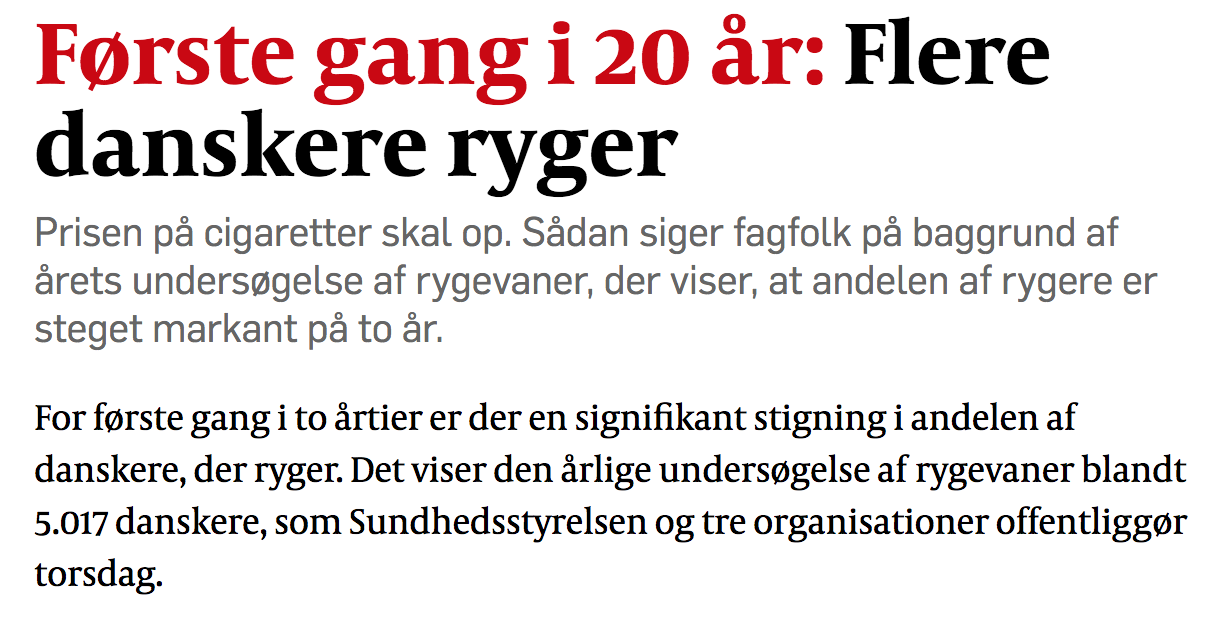
\includegraphics[scale=0.5]{rygere.png}
\end{frame}

%\begin{frame}{Jyllands Posten February 19 2019}
%\center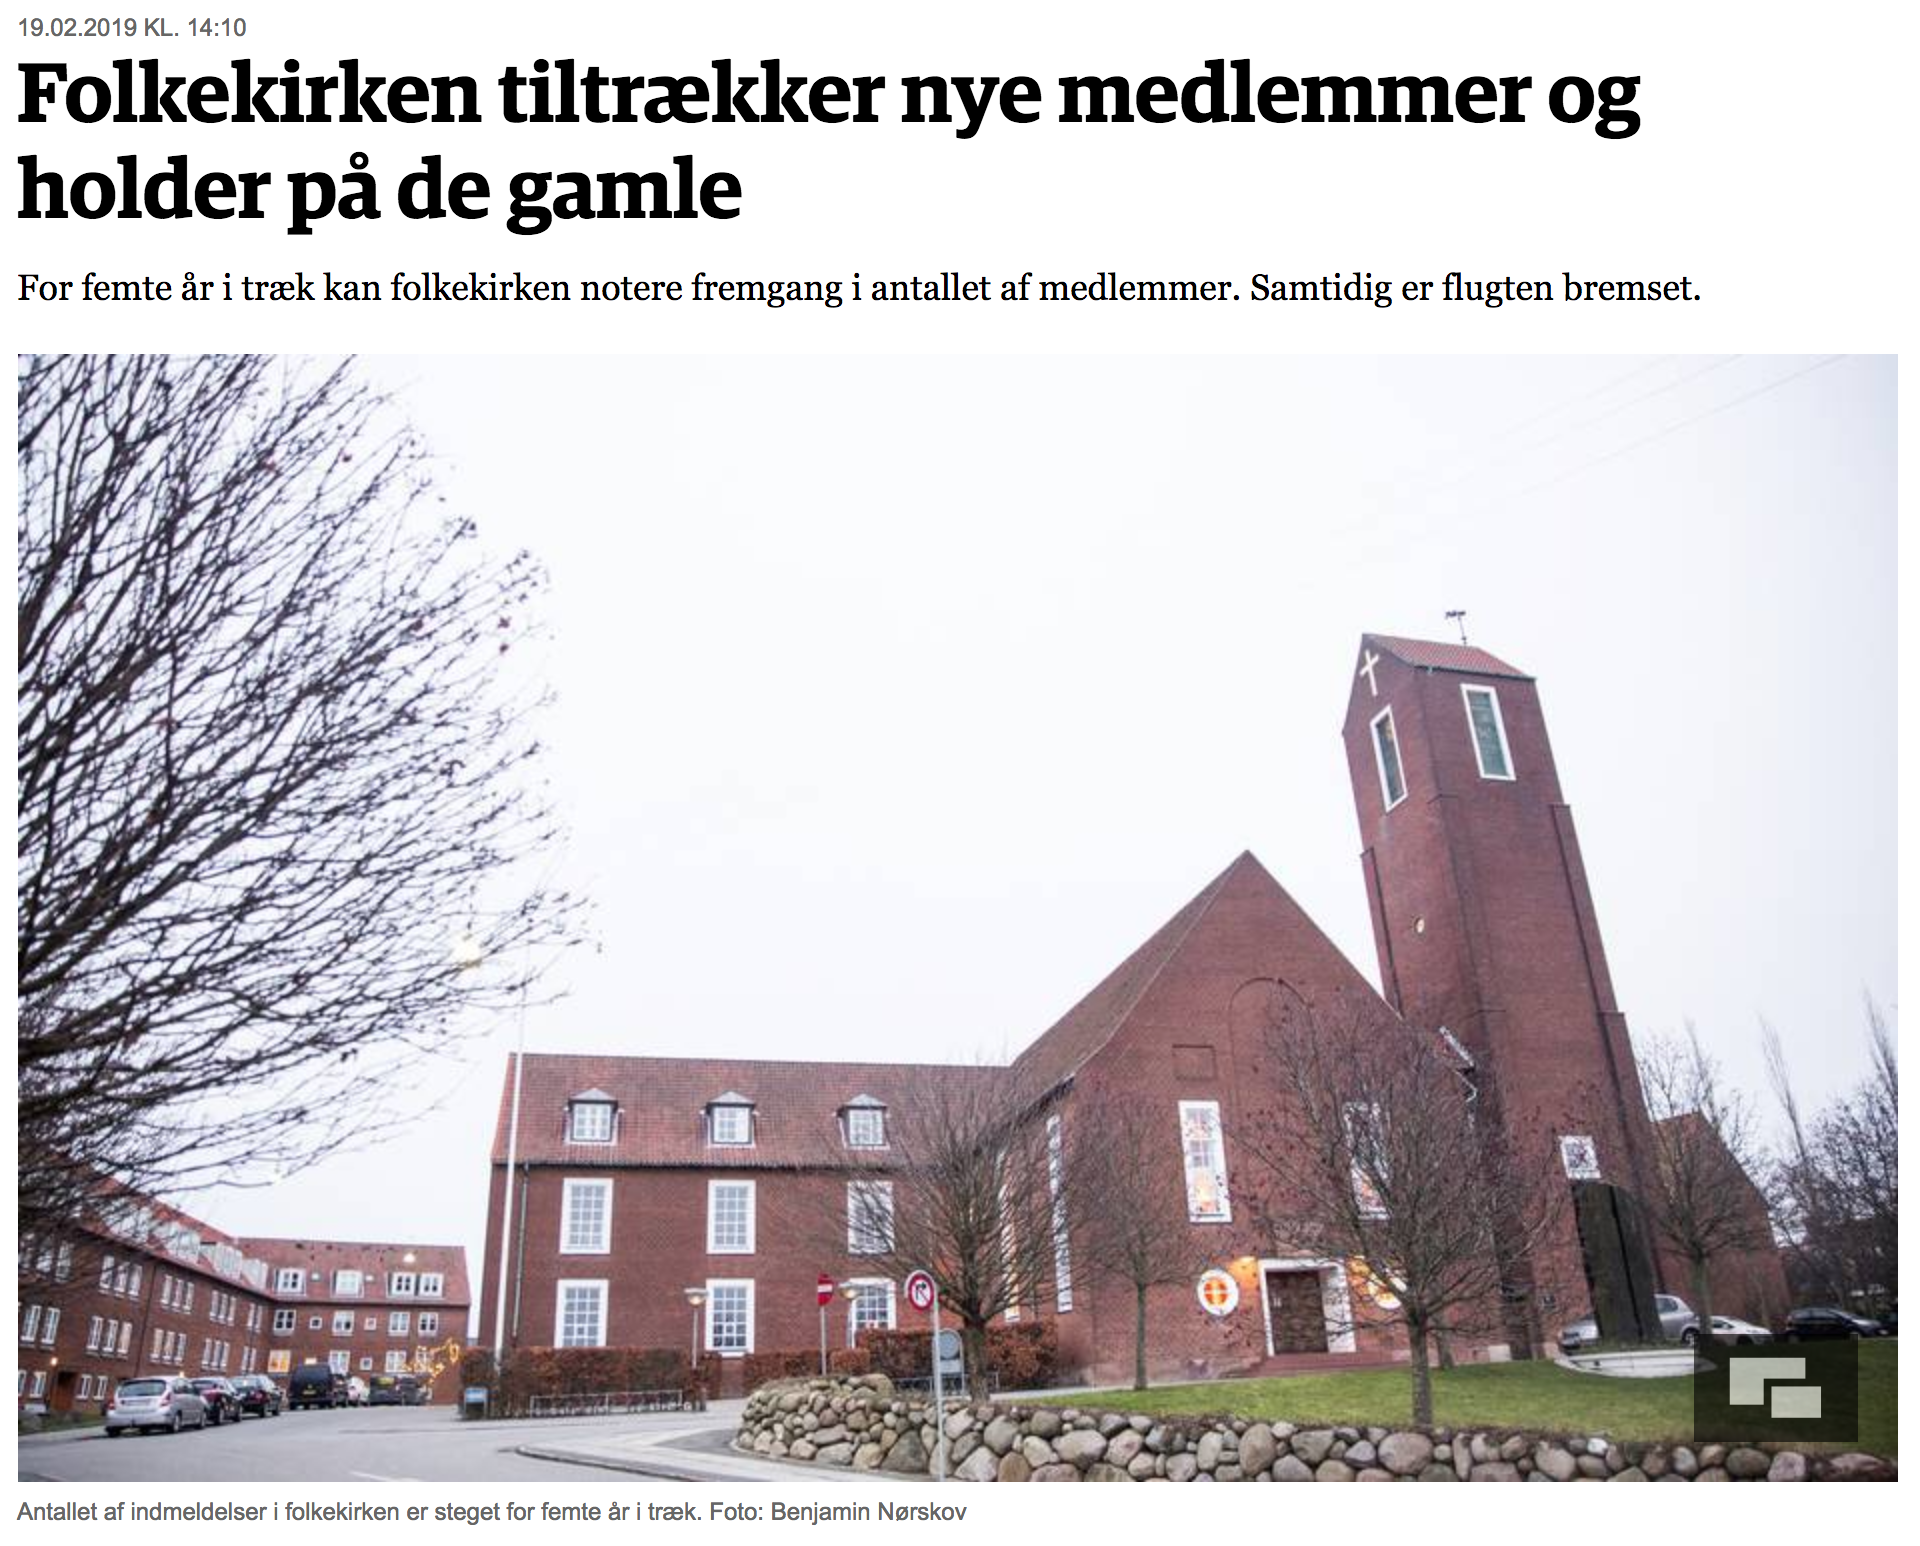
\includegraphics[scale=0.28]{baptisms.png}
%\end{frame}

\section{Five definitions}

\begin{frame}{Definition 1}
\begin{alertblock}{Definition 1}
  Reality evolves in continuous time $t \in \mathcal{T} \subset \mathbb{R}$.
\end{alertblock}  
\end{frame}


\begin{frame}{Definition 2}
\begin{alertblock}{Definition 2}
  There exists a random, latent function $f = \left\{f(t) : t \in \mathcal{T}\right\}$ governing the time evolution of some outcome. We can observe random variables sampled from $f$ at discrete time points with additive measurement noise
  \begin{align*}
	  Y_i &= f(t_i) + \varepsilon_i, \quad t_i \in \mathcal{T}, \quad \E[\varepsilon_i \mid t_i] = 0
  \end{align*}
  
  We are interested in understanding the dynamics of $f$ conditional on observed data $(Y_i, t_i)_{i=1}^{n}$.  
\end{alertblock}    
\end{frame}



\begin{frame}{Definition 3}
\begin{alertblock}{Definition 3}
  The \alert{trend} of $f$ is its instantaneous slope given by
  \begin{align*}
	  df(t) = \left(\frac{\mathrm{d} f(s)}{\mathrm{d}s}\right)(t)
  \end{align*}
  We say that $f$ exhibits a \alert{positive trend} at $t$ if $df(t) > 0$ and a \alert{negative trend} at $t$ if $df(t) < 0$.
\end{alertblock}    
\end{frame}



\begin{frame}{Definition 4}
\begin{alertblock}{Definition 4}
  A \alert{change in the trend} of $f$ is a point where $df$ changes sign (i.e., a positive trend becomes a negative trend or vice versa).
  
  \pause
 
  \vspace{1cm}
  
  A change in trend \alert{never} occurs at any given time point! It is a gradual and continuous event. The correct question is:
  \begin{quotation}
	  ,,What is the \alert{probability} that the trend is changing at time $t$ given what we have observed?''
  \end{quotation}
\end{alertblock}    
\end{frame}


\begin{frame}{Definition 5}
\begin{alertblock}{Definition 5}
  We define a local \alert{Trend Direction Index} as the conditional probability
  \begin{align*}
    \mathrm{TDI}(t, \delta) = P(df(t + \delta) > 0 \mid \mathcal{F}_t)
  \end{align*}
  where $\mathcal{F}_t$ is the sigma algebra of all available information up until time $t$.
\end{alertblock}    

\pause

\vspace{0.5cm}
\begin{itemize}
	\item{The sign of $\delta$ determines if we are estimating $(\delta \leq 0)$ or forecasting ($\delta > 0$).}
	\item{A similar index can be defined for $df(t + \delta) < 0$ but that is just $1 - \mathrm{TDI}(t, \delta)$ hence redundant.}
	\item{Examples in the public news are often with $t = \mathrm{now}$ and $\delta = 0$ (making change-point analyses impossible).}
\end{itemize}
\end{frame}



\section{Functional Data Approach}

\begin{frame}{Latent Gaussian Process model}
\begin{alertblock}{Gaussian Process}
A random function $\left\{f(t) : t \in \mathcal{T}\right\}$ is a Gaussian Process if and only if $(f(t_1), \ldots, f(t_n))$ has a multivariate normal distribution for every $(t_1, \ldots, t_n) \subset \mathcal{T}$ with $n < \infty$. $f \sim \mathcal{GP}(\mu(\cdot), C(\cdot, \cdot))$.
\end{alertblock}

\pause

\vspace{1cm}

We assume that the observed data is generated by the following hierarchical model:
\begin{align*}
  f \mid m, \theta &\sim \mathcal{GP}(m, C_\theta(\cdot,\cdot))\\
  Y_i \mid f(t_i), \Theta, t_i &\overset{iid}{\sim} N(f(t_i), \sigma^2), \quad \Theta = (m, \theta, \sigma^2)
\end{align*}
where $C_\theta\colon\, \mathcal{T} \times \mathcal{T} \mapsto \mathbb{R}$ is a parametric covariance function.
\end{frame}


\begin{frame}{Why a latent $\mathcal{GP}$?}
The conditional joint distribution of $(f, df)$ is a bivariate Gaussian Process:

\vspace{0.8cm}

\begin{align*}
  \begin{bmatrix}f(s)\\ df(t) \end{bmatrix} \mid m, \theta &\sim \mathcal{GP}\left(\begin{bmatrix}m\\ 0\end{bmatrix}, \begin{bmatrix}C_\theta(s, s^\prime) & \partial_2 C_\theta(s, t)\\ \partial_1 C_\theta(t, s) & \partial_1 \partial_2 C_\theta(t, t^\prime)\end{bmatrix}\right)
\end{align*}

\vspace{0.8cm}

Implication: We know the conditional distribution of $(f, df)$ at \alert{any} finite set of time point as well as their joint distribution with the observed data.

\end{frame}


\begin{frame}{Conditional joint distribution}
Let $\mathbf{Y}$ be the vector of random variables observed at time points $\mathbf{t}$ and $\mathbf{t}^\ast$ any finite subset of $\mathcal{T}$ not necessarily equal to $\mathbf{t}$. 

\vspace{1cm}

The conditional joint distribution of everything is then
{\footnotesize
\begin{align*}
  \begin{bmatrix}f(\mathbf{t}^\ast)\\ df(\mathbf{t}^\ast)\\ \mathbf{Y}\end{bmatrix} \mid \mathbf{t}, \Theta \sim N\left(\begin{bmatrix}m\\ 0\\ m\end{bmatrix}, \begin{bmatrix}C_\theta(\mathbf{t}^\ast,\mathbf{t}^\ast) & \partial_2 C_\theta(\mathbf{t}^\ast, \mathbf{t}^\ast) & C_\theta(\mathbf{t}^\ast, \mathbf{t})\\ \partial_1 C_\theta(\mathbf{t}^\ast, \mathbf{t}^\ast) &  \partial_1 \partial_2 C_\theta(\mathbf{t}^\ast, \mathbf{t}^\ast) & \partial_1 C_\theta(\mathbf{t}^\ast, \mathbf{t})\\ C_\theta(\mathbf{t}, \mathbf{t}^\ast) & \partial_2 C_\theta(\mathbf{t}, \mathbf{t}^\ast) & C_\theta(\mathbf{t}, \mathbf{t}) + \sigma^2 I\end{bmatrix}\right)
\end{align*}
}%
\end{frame}



\begin{frame}{Conditional joint posterior distribution}
Directly the joint conditional posterior distribution of the latent functions is
\begin{align*}
\begin{bmatrix}f(\mathbf{t}^\ast)\\ df(\mathbf{t}^\ast) \end{bmatrix} \mid \mathbf{Y}, \mathbf{t}, \Theta &\sim
N\left(\begin{bmatrix}\mu_f(\mathbf{t}^\ast)\\ \mu_{df}(\mathbf{t}^\ast)\end{bmatrix}, \begin{bmatrix}\Sigma_{f,f}(\mathbf{t}^\ast, \mathbf{t}^\ast) & \Sigma_{f,df}(\mathbf{t}^\ast, \mathbf{t}^\ast)\\ \Sigma_{f,df}(\mathbf{t}^\ast, \mathbf{t}^\ast)^T & \Sigma_{df,df}(\mathbf{t}^\ast, \mathbf{t}^\ast)\end{bmatrix}\right)
\end{align*}

{\footnotesize
\begin{align*}
  \mu_f(\mathbf{t}^\ast) &= m + C_\theta(\mathbf{t}^\ast, \mathbf{t})\left[C_\theta(\mathbf{t}, \mathbf{t}) + \sigma^2 I\right]^{-1}\left(\mathbf{Y} - m\right)\nonumber\\
  \mu_{df}(\mathbf{t}^\ast) &= \partial_1 C_\theta(\mathbf{t}^\ast, \mathbf{t})\left[C_\theta(\mathbf{t}, \mathbf{t}) + \sigma^2 I\right]^{-1}\mathbf{Y}\nonumber\\
  \Sigma_{f,f}(\mathbf{t}^\ast, \mathbf{t}^\ast) &= C_\theta(\mathbf{t}^\ast, \mathbf{t}^\ast) - C_\theta(\mathbf{t}^\ast, \mathbf{t})\left[C_\theta(\mathbf{t}, \mathbf{t}) + \sigma^2 I\right]^{-1} C_\theta(\mathbf{t}^\ast, \mathbf{t})^T\nonumber\\
  \Sigma_{df,df}(\mathbf{t}^\ast, \mathbf{t}^\ast) &= \partial_1 \partial_2 C_\theta(\mathbf{t}^\ast, \mathbf{t}^\ast) - \partial_1 C_\theta(\mathbf{t}^\ast, \mathbf{t})\left[C_\theta(\mathbf{t}, \mathbf{t}) + \sigma^2 I\right]^{-1} \partial_1 C_\theta(\mathbf{t}^\ast, \mathbf{t})^T\nonumber\\
  \Sigma_{f,df}(\mathbf{t}^\ast, \mathbf{t}^\ast) &= \partial_1 C_\theta(\mathbf{t}^\ast, \mathbf{t}^\ast) - C_\theta(\mathbf{t}^\ast, \mathbf{t})\left[C_\theta(\mathbf{t}, \mathbf{t}) + \sigma^2 I\right]^{-1}\partial_1 C_\theta(\mathbf{t}^\ast, \mathbf{t})^T\nonumber
\end{align*}
}%
\end{frame}


\begin{frame}{Example}
Let's see what this looks like on $\mathcal{T} = [0;1]$ in the noise-free case ($\sigma^2 = 0$) with known parameters.
  
We use the exponential squared covariance function
\begin{align*}
  C_\theta(s,t) = \alpha^2 \exp\left(-\frac{(s-t)^2}{2\rho^2}\right), \quad \theta = (\alpha, \rho)
\end{align*}
where $\alpha$ is the standard deviation of the latent function and $\rho$ is its \textit{length-scale}. We set $\alpha = 2$ and $\rho = 0.1$.
\end{frame}

\begin{frame}{Example - prior distribution of $f$}
  What the world looks like without observed data
  \center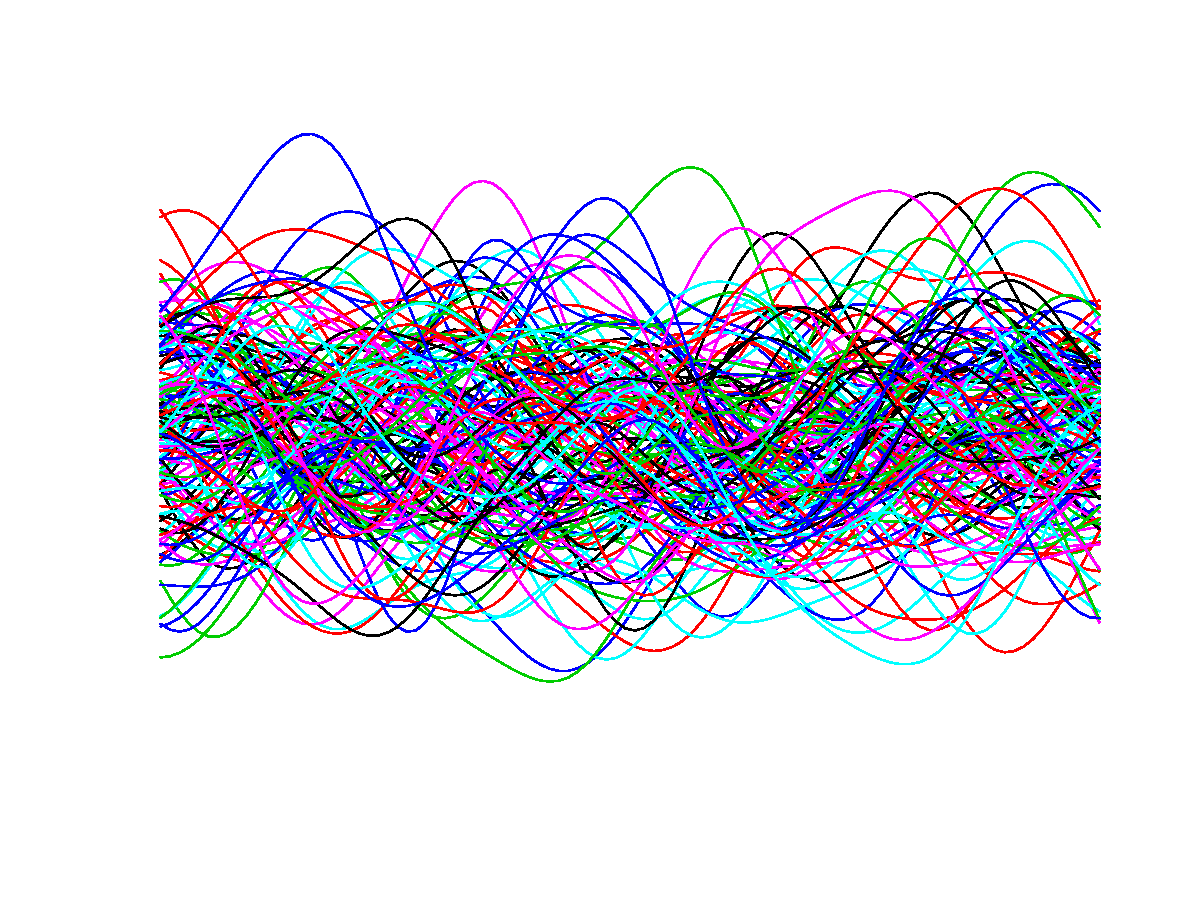
\includegraphics[scale=0.5]{postAni01}
\end{frame}

\begin{frame}{Example - posterior distribution of $(f, df)$}
  Posterior distributions conditional on 1 observation
  \center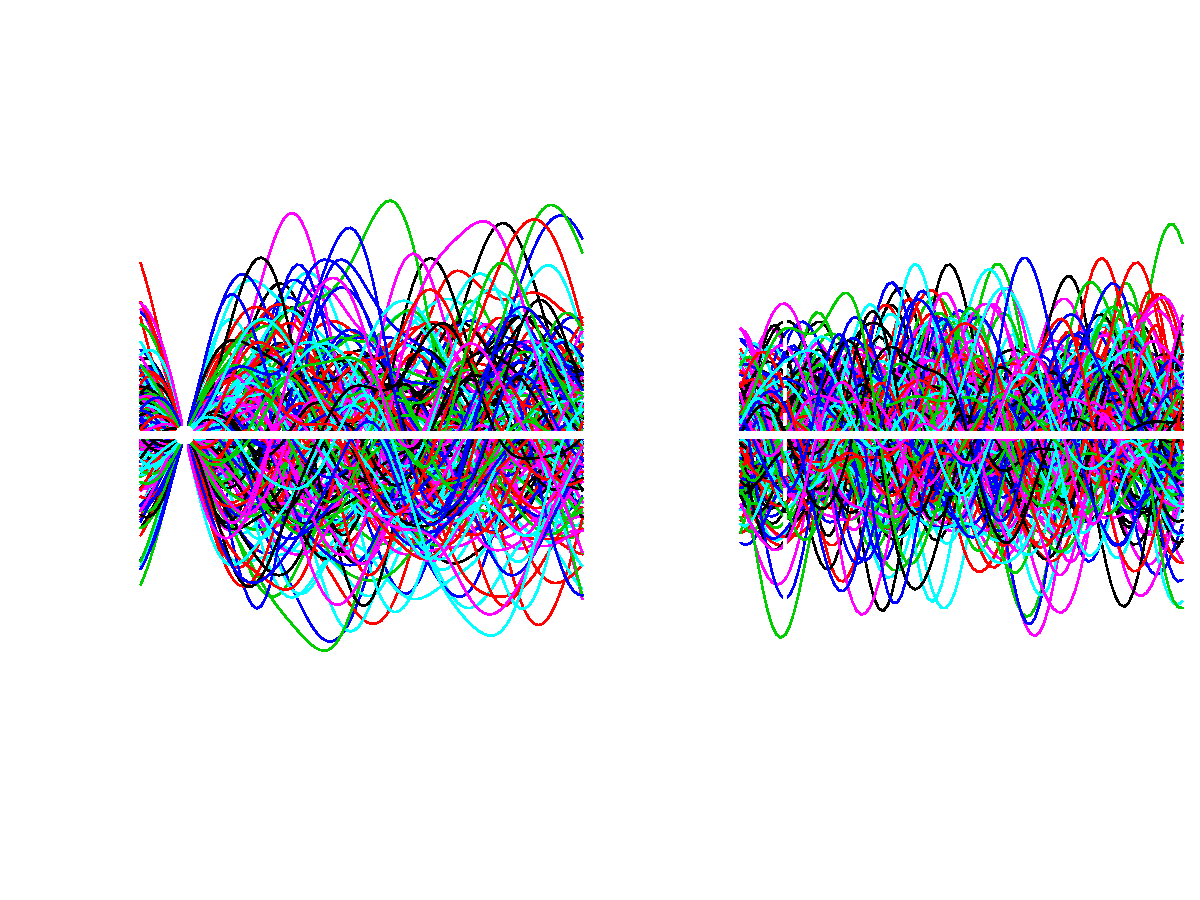
\includegraphics[scale=0.5]{postAni02}
\end{frame}

\begin{frame}{Example - posterior distribution of $(f, df)$}
  Posterior distributions conditional on 2 observations
  \center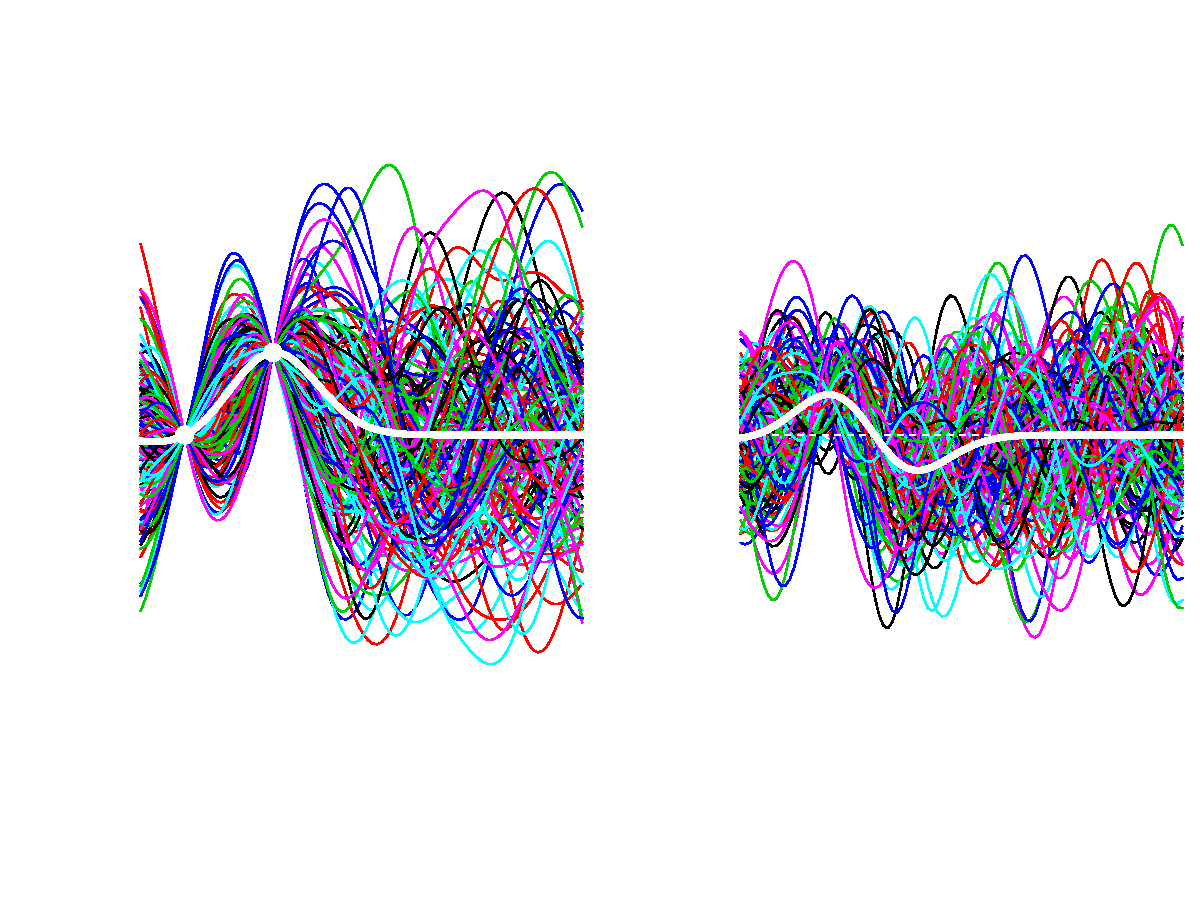
\includegraphics[scale=0.5]{postAni03}
\end{frame}

\begin{frame}{Example - posterior distribution of $(f, df)$}
  Posterior distributions conditional on 3 observations
  \center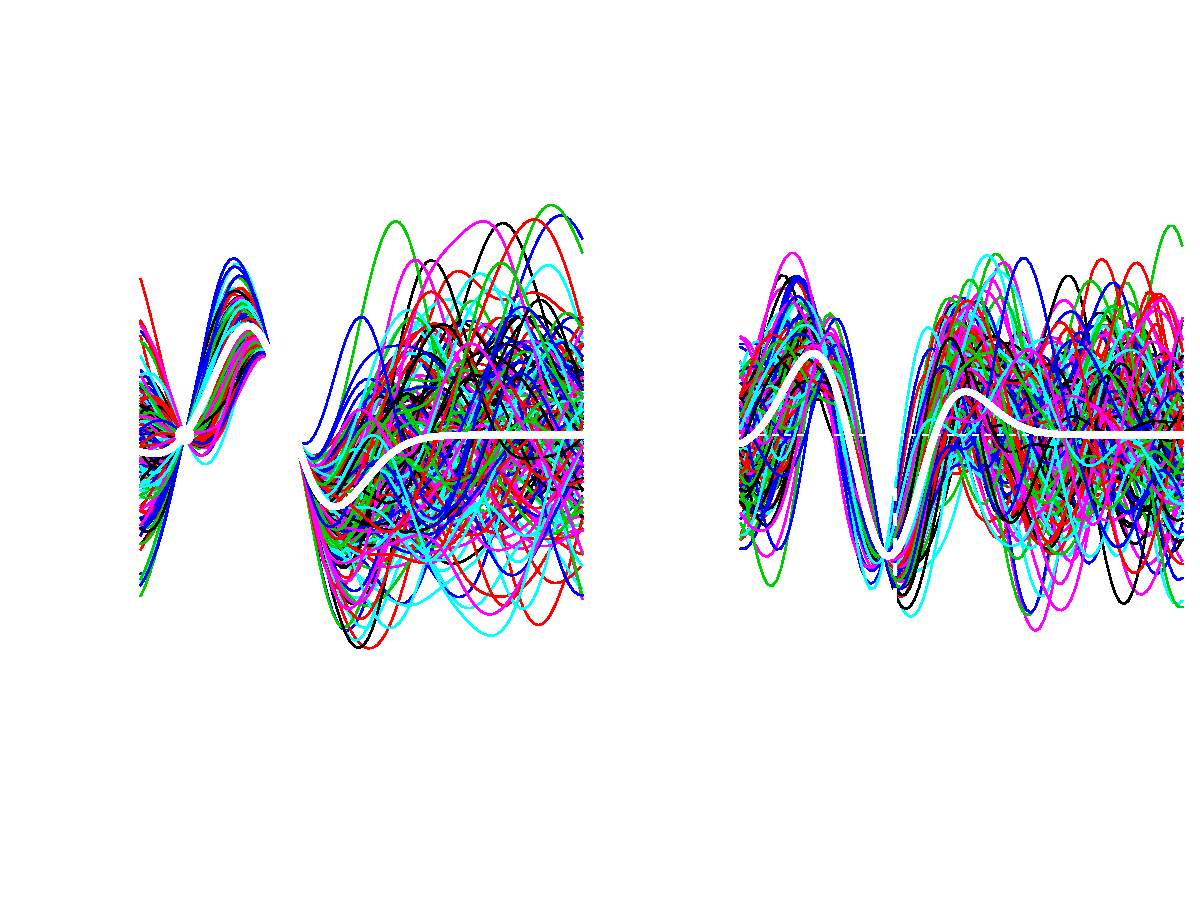
\includegraphics[scale=0.5]{postAni04}
\end{frame}

\begin{frame}{Example - posterior distribution of $(f, df)$}
  Posterior distributions conditional on 4 observations
  \center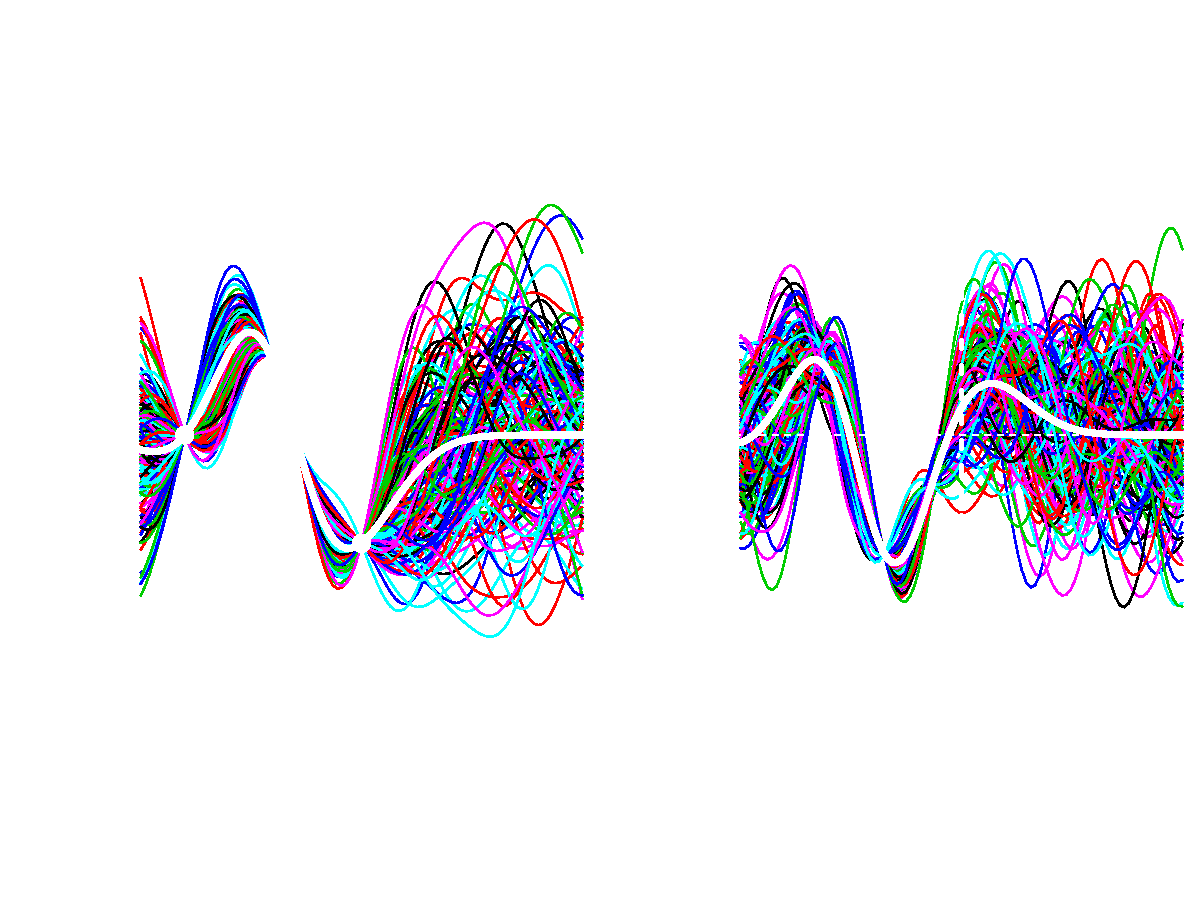
\includegraphics[scale=0.5]{postAni05}
\end{frame}

\begin{frame}{Example - posterior distribution of $(f, df)$}
  Posterior distributions conditional on 5 observations
  \center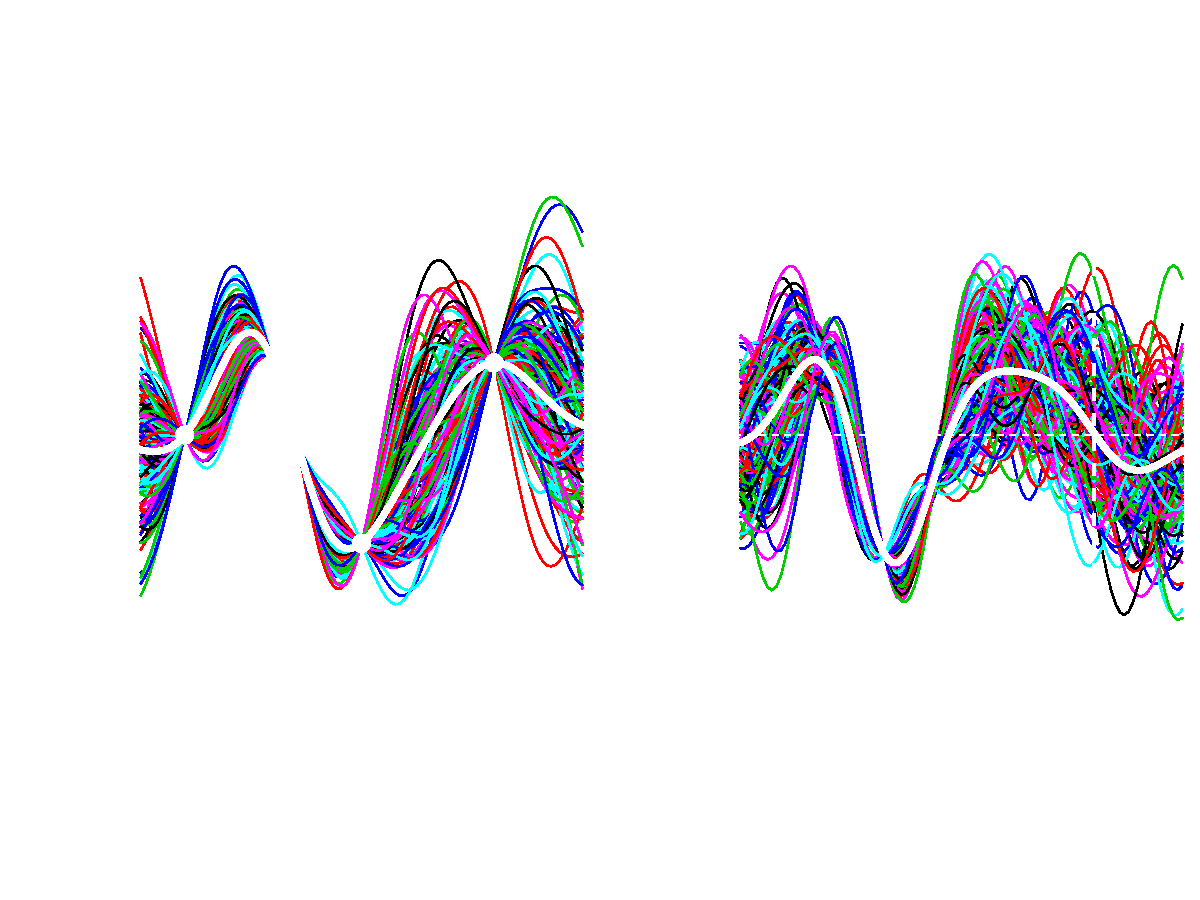
\includegraphics[scale=0.5]{postAni06}
\end{frame}

\begin{frame}{Example - posterior distribution of $(f, df)$}
  Posterior distributions conditional on 6 observations
  \center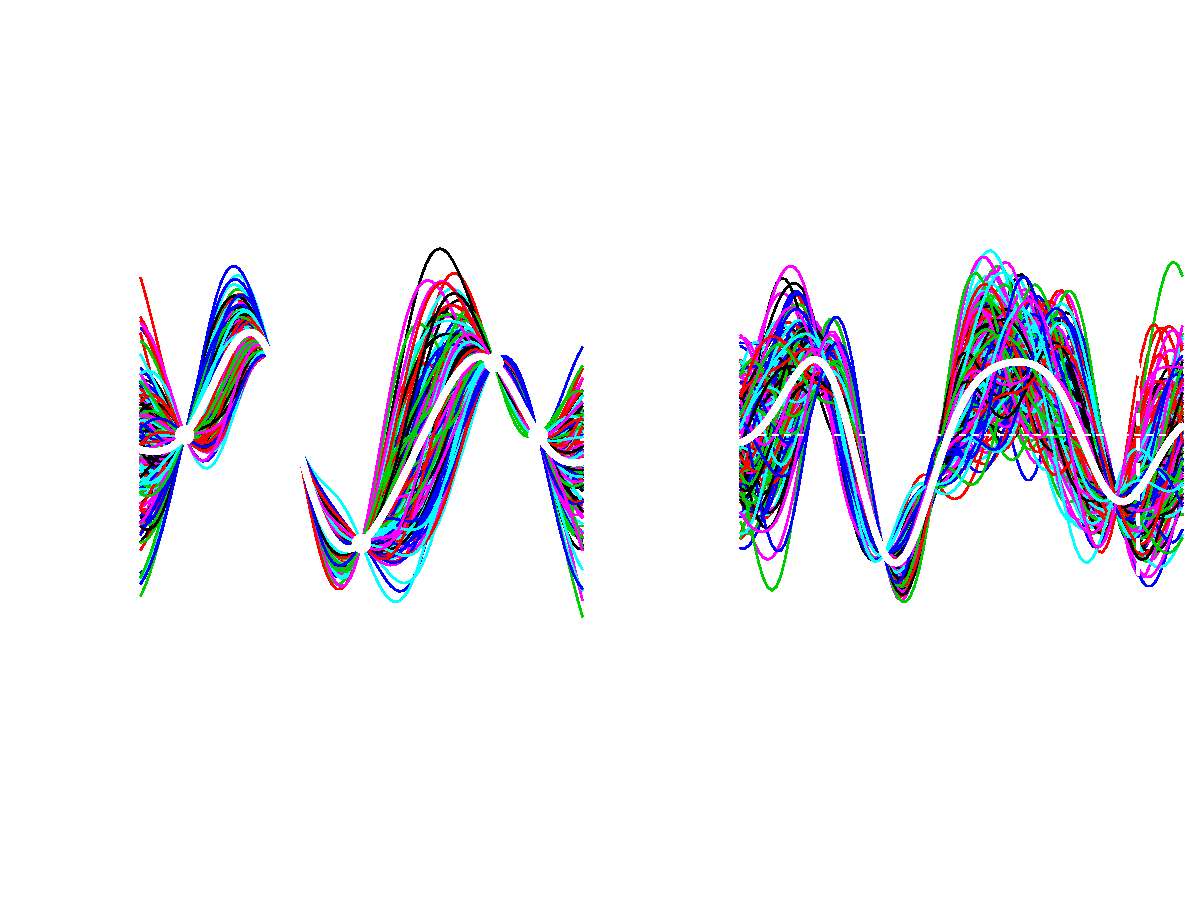
\includegraphics[scale=0.5]{postAni07}
\end{frame}


\begin{frame}{Trend Direction Index}
Recall the definition of the Trend Direction Index
\begin{align*}
  \mathrm{TDI}(t, \delta) = P(df(t + \delta) > 0 \mid \mathcal{F}_t)	
\end{align*}
Letting $\mathcal{F}_t$ be generated by $\left\{\mathbf{Y}, \mathbf{t}\right\}$, we may express the \alert{Trend Direction Index} as
\begin{align*}
  \mathrm{TDI}(t, \delta \mid \Theta) &= P\left(df(t + \delta) > 0 \mid \mathbf{Y}, \mathbf{t}, \Theta\right)\\
        &= \int_0^\infty N\left(u, \mu_{df}(t + \delta), \Sigma_{df,df}(t + \delta,t + \delta)^{1/2}\right)\mathrm{d}u
\end{align*}
\end{frame}


\begin{frame}{Example - posterior distribution of $f$ and TDI}
  \center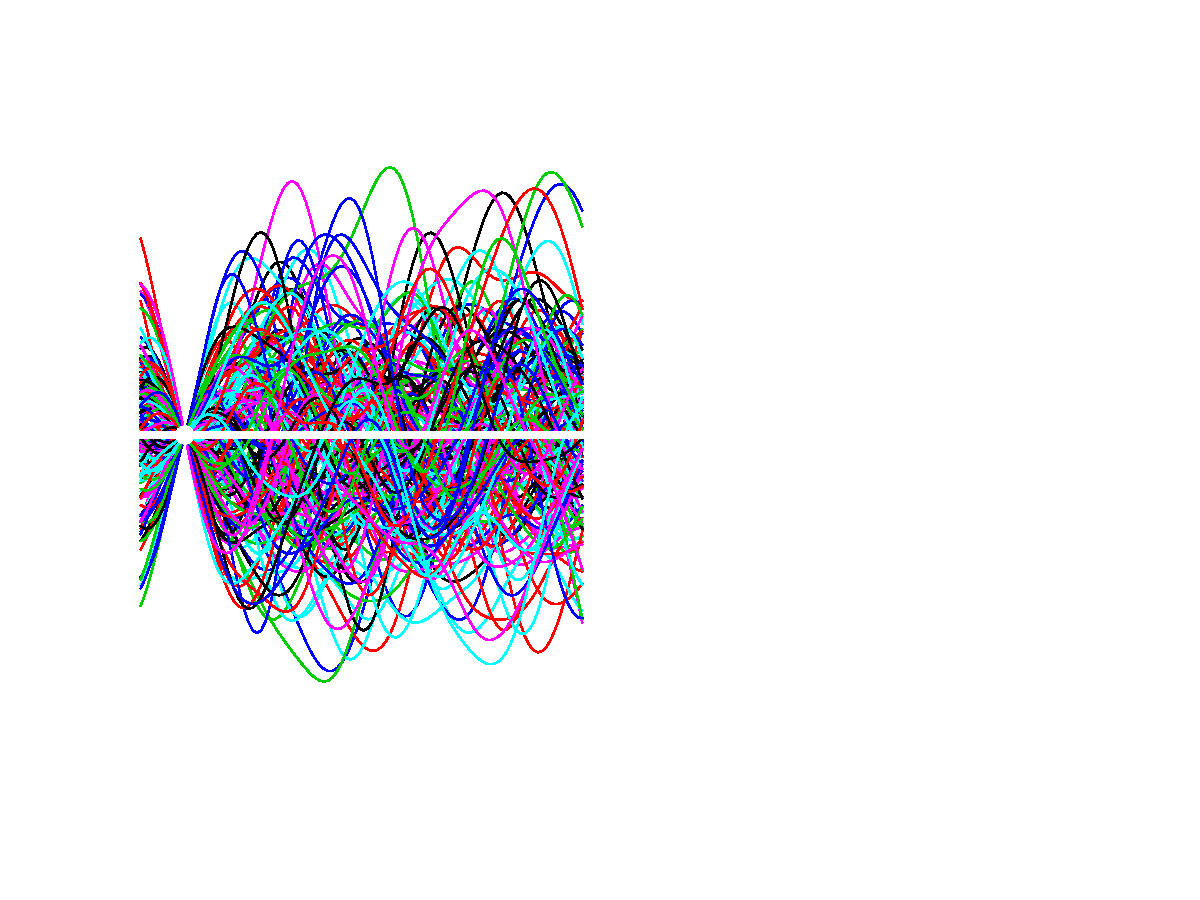
\includegraphics[scale=0.5]{probAni01}
\end{frame}
\begin{frame}{Example - posterior distribution of $f$ and TDI}
  \center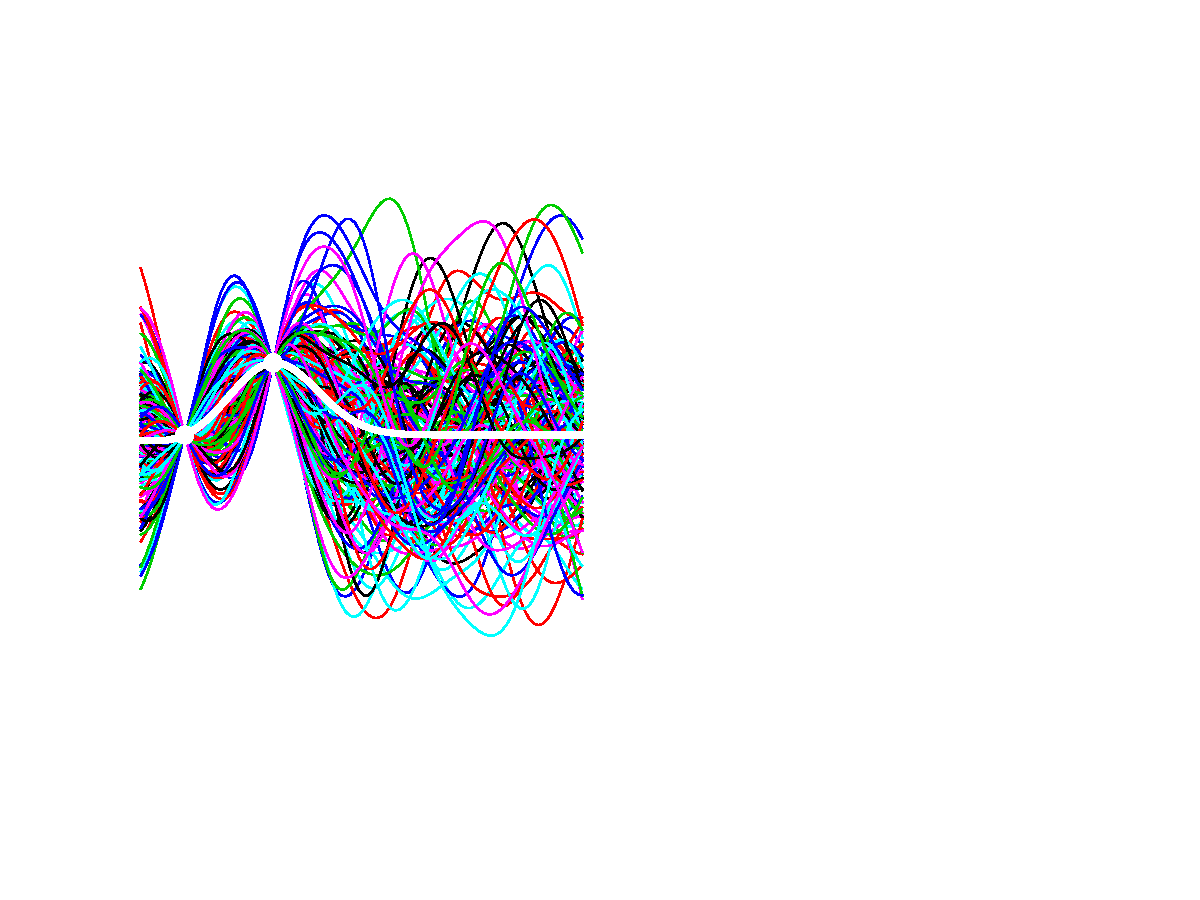
\includegraphics[scale=0.5]{probAni02}
\end{frame}
\begin{frame}{Example - posterior distribution of $f$ and TDI}
  \center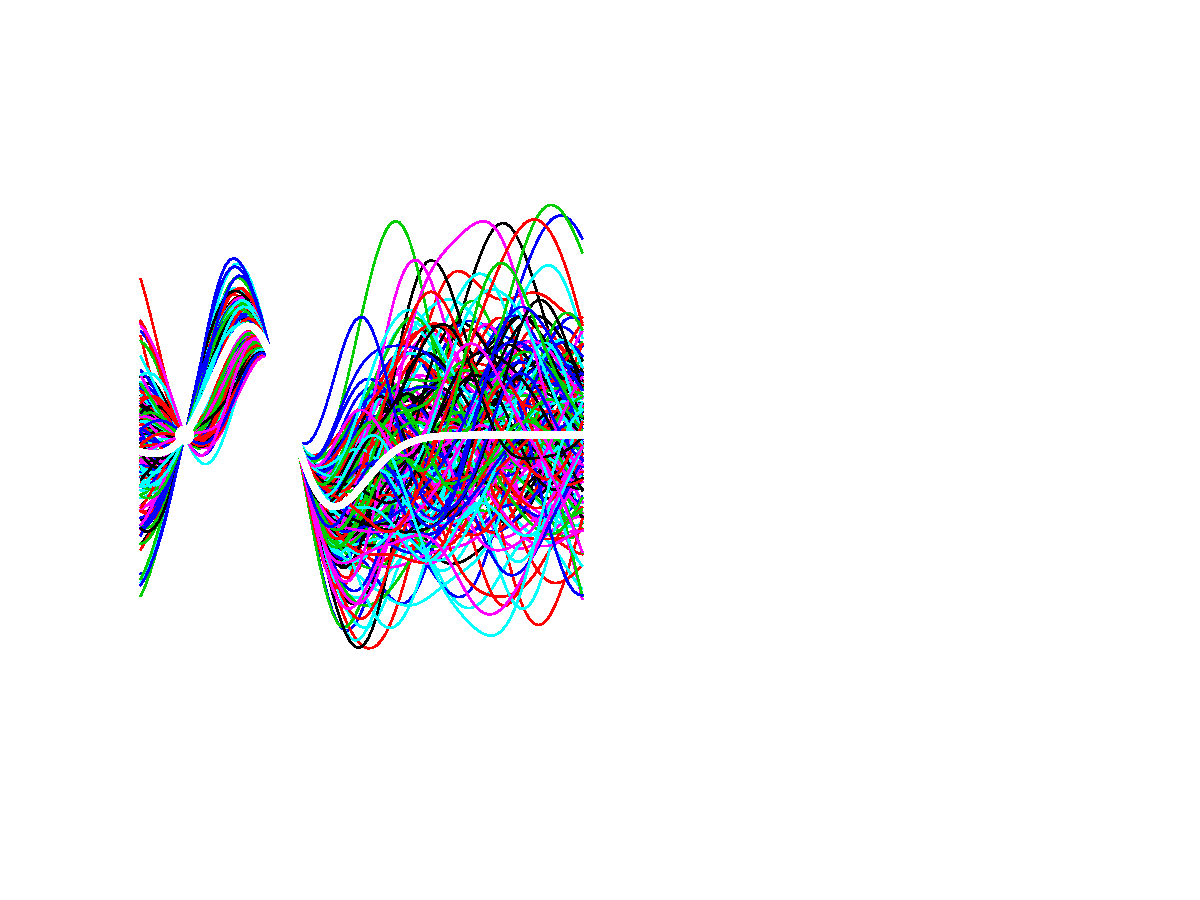
\includegraphics[scale=0.5]{probAni03}
\end{frame}
\begin{frame}{Example - posterior distribution of $f$ and TDI}
  \center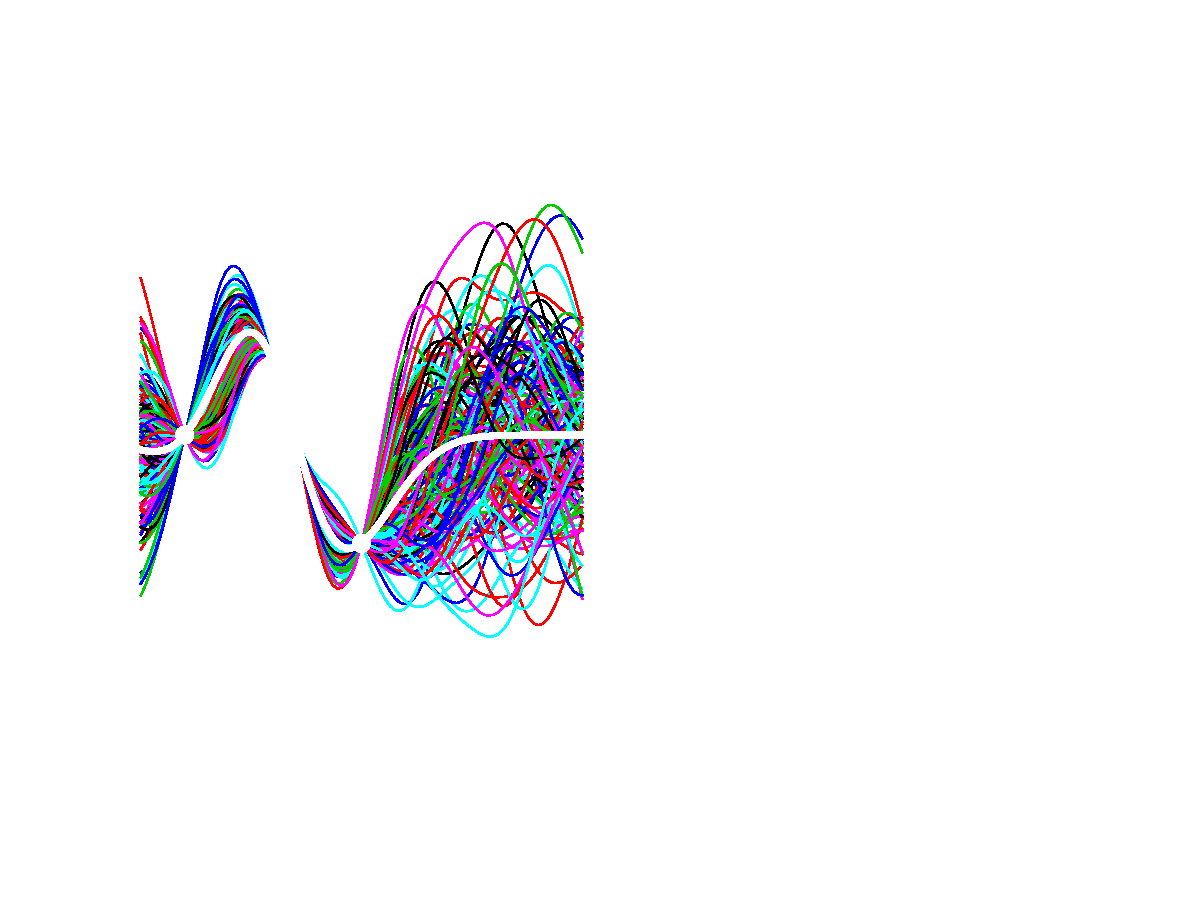
\includegraphics[scale=0.5]{probAni04}
\end{frame}
\begin{frame}{Example - posterior distribution of $f$ and TDI}
  \center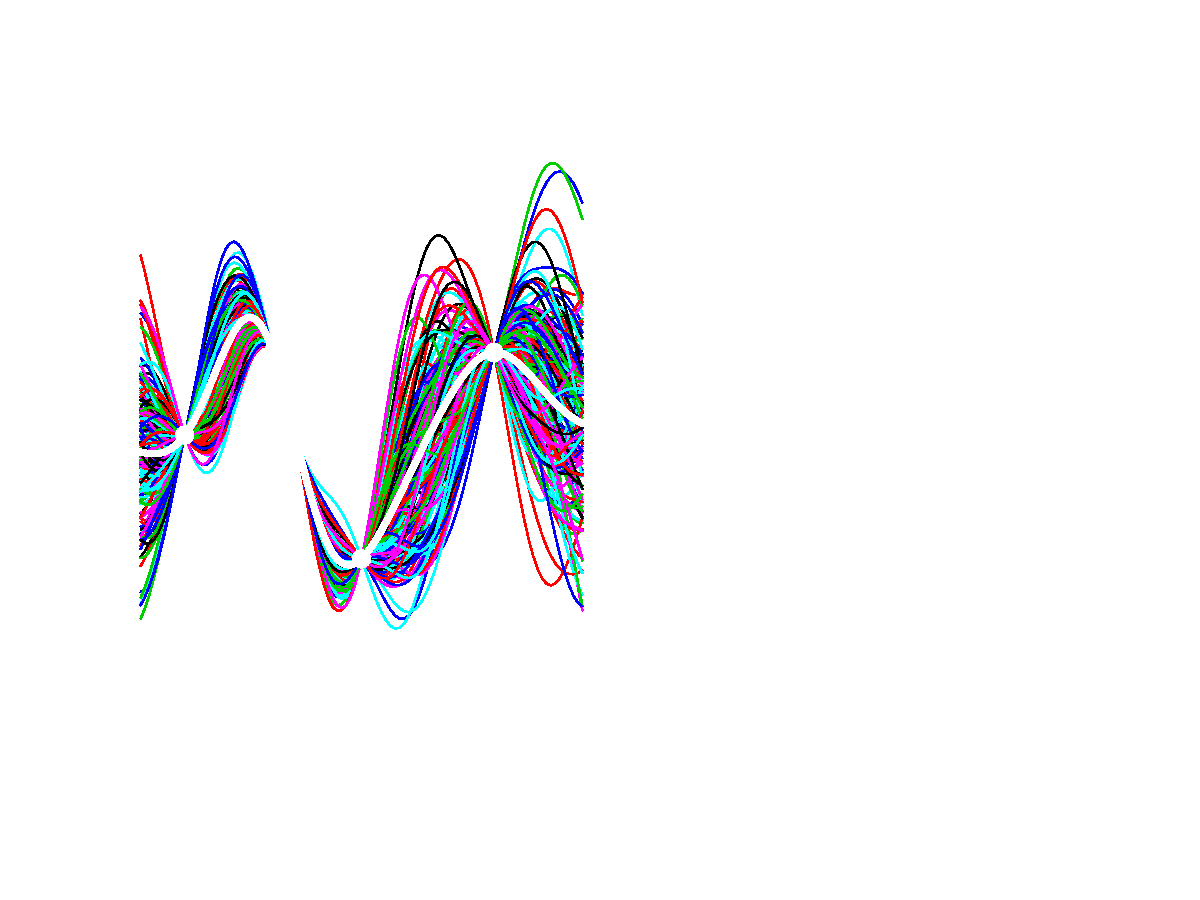
\includegraphics[scale=0.5]{probAni05}
\end{frame}
\begin{frame}{Example - posterior distribution of $f$ and TDI}
  \center
\includegraphics[scale=0.5]{probAni06}
\end{frame}


\section{Estimation}

\begin{frame}{Two approaches}
\begin{itemize}
  \item{\textbf{Empirical Bayes estimation}}
  \begin{itemize}
	  \item[\Fire]{Maximize the marginal likelihood and plug-in}
	  \item[\Fire]{$\widehat{\Theta} = \argsup_{\Theta} \log L(\mathbf{Y} \mid \mathbf{t}, \Theta)$ and $\mathrm{TDI}(t, \delta \mid \widehat{\Theta})$}
	  \item[\Smiley]{Fast and easy to implement}
	  \item[\Xey]{Can only be used in a very simple models where the marginal likelihood is analytically available}
	  \item[\Xey]{Does not account for the uncertainty in $\Theta$}
  \end{itemize}
  \pause
  
  \vspace{1cm}
  
  \item{\textbf{Fully Bayesian estimation}}
  \begin{itemize}
	  \item[\Fire]{Markov chain Monte Carlo estimation with priors on $\Theta$}
	  \item[\Smiley]{Easily extendable to more complex models}
	  \item[\Smiley]{Accounts for all the uncertainty in the model. $\mathrm{TDI}(t, \delta \mid \Theta)$ is now a distribution over probabilities}
	  \item[\fryingpan]{Requires special implementions or... \alert{\textbf{Stan}}!}
  \end{itemize}
\end{itemize}
\end{frame}

\begin{frame}[fragile]{Fully Bayesian estimation in Stan}
\begin{columns}
\begin{column}{0.5\textwidth}
\begin{Verbatim}[fontsize=\footnotesize]
functions {
}

data {
}

parameters {
}

transformed parameters {
}

model {
}

generated quantities {
}
\end{Verbatim}
\end{column}
\begin{column}{0.5\textwidth}  %%<--- here
\begin{center}
  
\includegraphics[width=0.5\textwidth]{logo_tm}
  \texttt{https://mc-stan.org/}
\end{center}
\end{column}
\end{columns}
\end{frame}


\begin{frame}[fragile]{The Stan program 1/2}
\begin{Verbatim}[fontsize=\scriptsize]
functions{
  matrix pred_rng(real[] xPred, vector y, real[] x, real m, 
                  real alpha, real rho, real sigma) {
    //...
  }	
}

data {
  int<lower = 1> n;
  real x[n];
  vector[n] y;
  int<lower = 1> nPred;
  real xPred[nPred];
}

parameters {
  real mu;
  real<lower = 0> alpha;  
  real<lower = 0> rho;
  real<lower = 0> sigma;
}
\end{Verbatim}
\end{frame}


\begin{frame}[fragile]{The Stan program 2/2}
\begin{Verbatim}[fontsize=\scriptsize]
model {
  matrix[n, n] K = cov_exp_quad(x, alpha, rho);
  for (i in 1:n) {
    K[i, i] = K[i, i] + square(sigma);
  }
  
  mu ~ normal(26.835, 3);
  alpha ~ normal(0, 3);
  rho ~ inv_gamma(3.548762, 10.221723); // <- what is this?
  sigma ~ normal(0, 3);

  y ~ multi_normal_cholesky(rep_vector(mu, n), cholesky_decompose(K));
}

generated quantities {
  matrix[nPred, 4] pred;
  pred = pred_rng(xPred, y, x, mu, alpha, rho, sigma);
}
\end{Verbatim}
\end{frame}


\section{Application}

\begin{frame}{From the Danish Health Authority\footnotemark}
\center
\includegraphics[scale=0.38]{rygereSST1.png}
\center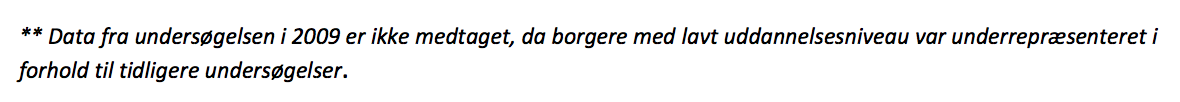
\includegraphics[scale=0.42]{rygereSST2.png}
\center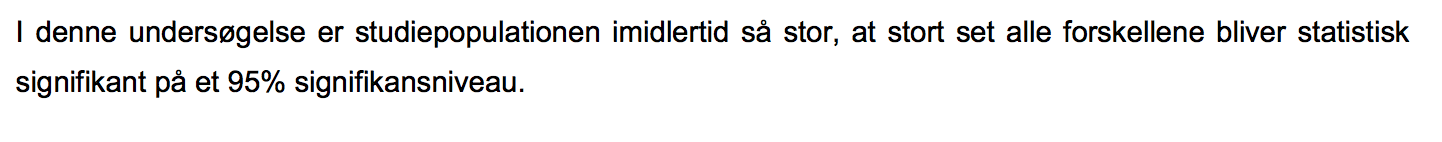
\includegraphics[scale=0.344]{rygereSST3.png}
\footnotetext[1]{\tiny Nøgletal - Danskernes rygevaner 2018, \texttt{www.sst.dk/da/udgivelser/2019/danskernes-rygevaner-2018}}
\end{frame}


\begin{frame}{Proportion of smokers in Denmark}
\center
\includegraphics[scale=0.5]{smokersData}
\end{frame}

\begin{frame}{Model fit}
  \center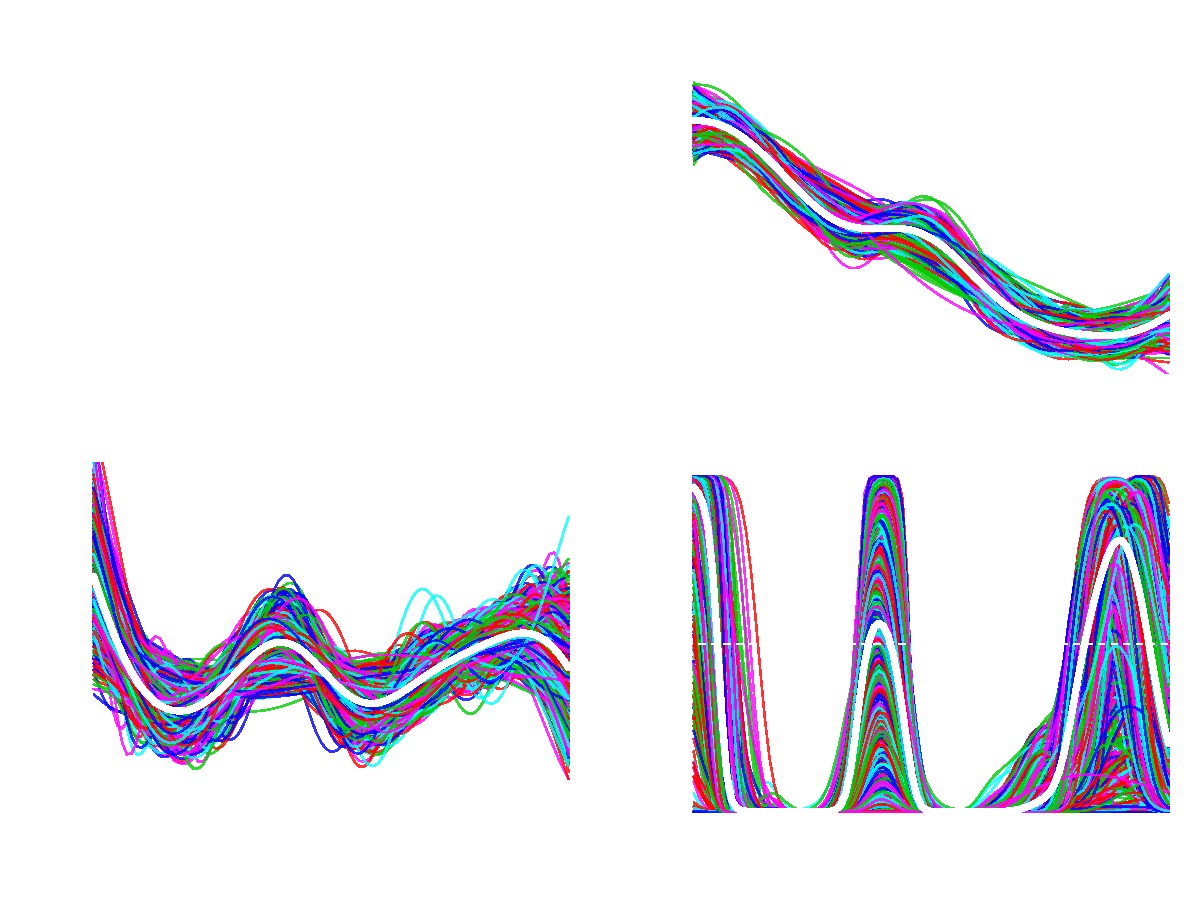
\includegraphics[scale=0.5]{smoking1}
\end{frame}



\section{Extensions}

\begin{frame}
\center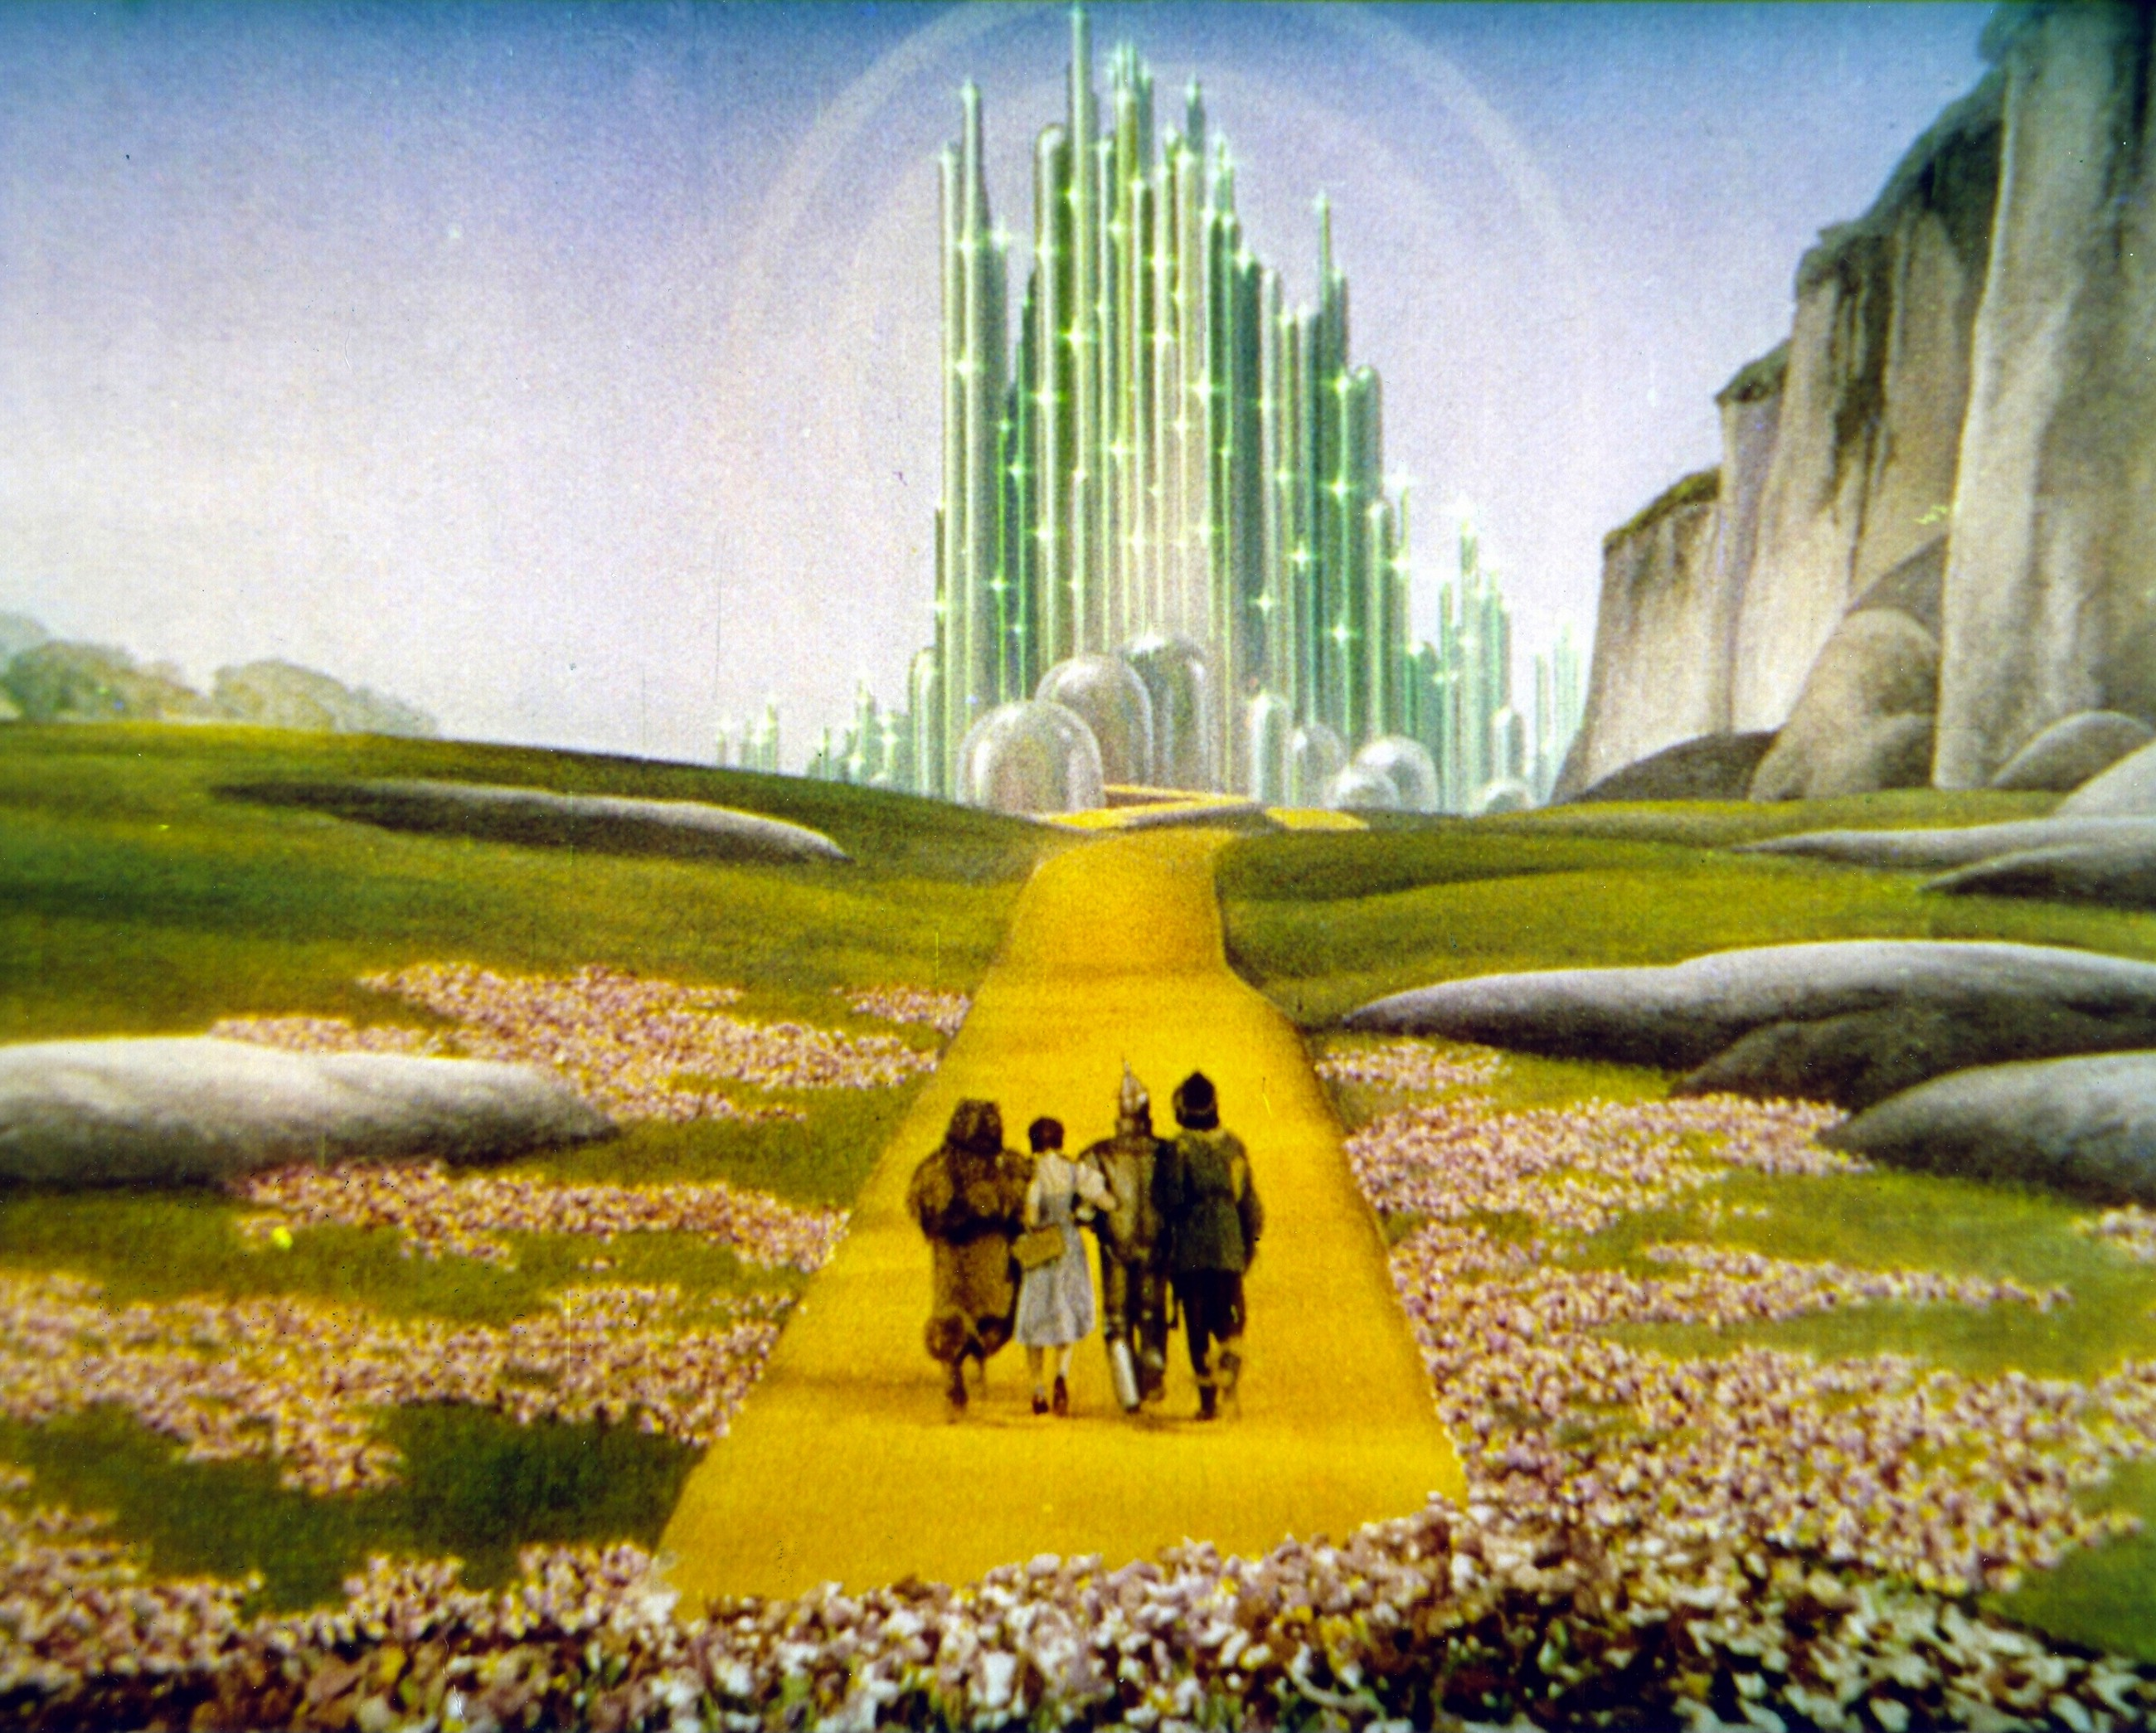
\includegraphics[scale=0.1175]{ybr.jpeg}
\end{frame}

\begin{frame}{Stationarity and latent dynamics}
A stationary covariance function $C_\theta(s,t) = C_\theta(|s-t|)$ is often used out of convenience. In the previous model we used the exponential squared covariance function. It can be shown that $\partial_2 C_\theta(t,t) = 0$ for all stationary covariance functions hence $f(t) \independent df(t)$.

\pause

\vspace{0.8cm}

By construction $df(t) \mid f(t), \Theta = \alpha(t) + \beta(t)f(t) + \epsilon(t)$ and therefore $\beta(t) = 0$ imposing a strong assumption on the latent dynamics.

\vspace{0.8cm}

To obtain $\beta(t) \ne 0$ we must enable non-stationarity. This can be achived flexibly by adding a functional latent class to the model.
\end{frame}

\begin{frame}{Functional latent class model extension}
We add a time-varying latent class as follows
\begin{align*}
  w(t) \mid \phi &\sim S_{K-1}^\infty(\phi)\\
  G(t) \mid w(t), \phi &\sim \Multinomial(w(t))\\
  f(t) \mid G(t) = k, \theta_k, \mathbf{w}, \phi &\sim \mathcal{GP}(m, C_{\theta_k}(\cdot,\cdot))
\end{align*}
where $S_{K-1}^\infty$ is a distribution on the functional $K-1$ dimensional simplex
\begin{align*}
  \left\{w_k(t), k = 1,\ldots, K, t \in \mathcal{T}, w_k(t) > 0, \sum_{k=1}^K w_k(t) = 1\right\}
\end{align*}
\end{frame}


\begin{frame}{Functional latent class model extension}
Marginalizing out $G(t)$ we obtain
\begin{align*}
  \begin{bmatrix}f(s)\\ df(t) \end{bmatrix} \mid m, \left\{w_k, \theta_k\right\}_{k=1}^K, \phi &\sim \mathcal{GP}\left(\begin{bmatrix}m\\ 0\end{bmatrix}, \begin{bmatrix}C_{11}(s, s^\prime) & C_{12}(s, t)\\ C_{21}(t, s) & C_{22}(t, t^\prime)\end{bmatrix}\right)
\end{align*}
where
\begin{align*}
  C_{11}(s, s^\prime) &= \sum_{k=1}^K w_k(s)C_{\theta_k}(s,s^\prime)w_k(s^\prime)\\
  C_{12}(s, t) &= \partial_2 C_{11}(s, t)\\
               &= \sum_{k=1}^K w_k(s) \partial_2 C_{\theta_k}(s,t)w_k(t) + \sum_{k=1}^K w_k(s)C_{\theta_k}(s,t)dw_k(t)
\end{align*}
and $C_{12}(t,t)$ is now generally non-zero and therefore conditionally $df(t) \not\!\perp\!\!\!\perp f(t)$.
\end{frame}

\begin{frame}{Applying the non-stationary model}
We use $K = 2$ hence $\mathbf{w}(t) = (w_1(t), 1 - w_1(t))$.
  
We model $w_1(t)$ by a transformed polynomial B-spline expansion with $P = 15$
\begin{align*}
  w_1(t) = \logit^{-1}\left(\phi_0 + \sum_{p=1}^P \phi_p B(t)\right)
\end{align*}
and regularize by an autogressive prior
\begin{align*}
   \phi_1 \sim N(0,1), \quad \phi_{p} \sim N(\phi_{p-1}, \tau), \quad \tau \sim N(0, 1)
\end{align*}
Its derivative then has the closed form expression
\begin{align*}
  dw_1(t) &= \left(\sum_{p=1}^P \phi_p \frac{\mathrm{d}}{\mathrm{dt}}B_p(t)\right) \mathrm{d}\logit^{-1}(t)\left(\phi_0 + \sum_{p=1}^P \phi_p B_p(t)\right)
\end{align*}
\end{frame}

\begin{frame}{Latent class fit}
\center
\includegraphics[scale=0.5]{smoking2-1}
\end{frame}


\begin{frame}{A useful link}
%\texttt{https://github.com/aejensen/gptrendR}

%R implementation of the basic model using Empirical Bayes estimation.

%\vspace{1cm}

\texttt{https://github.com/aejensen/TrendinessOfTrends}

\begin{itemize}
  \item[\Coffeecup]{Stan implementations}
  \item[\Coffeecup]{Data and code to reproduce the figures}
  \item[\Coffeecup]{Work-in-progress preprint of the manuscript}
  \item[\Coffeecup]{These slides}
\end{itemize}

%\vspace{1cm}
%\texttt{https://github.com/aejensen/gptrendR}
%\begin{itemize}
%  \item[\Coffeecup]{R package implementing Empirical Bayes estimation for the model without latent classes}
%\end{itemize}
\end{frame}



\begin{frame}
\center \Huge Thank you!
\end{frame}

\end{document}

